\documentclass[titlepage]{report}
\title{EC2-virtual-server und EC2-container in der Amazon AWS Cloud \\
\large Eine Seminar-Arbeit bei Prof. Dr. -Ing. Dr. rer. nat. habil. \\
Harald Richter}
\usepackage[ngerman]{babel}
\usepackage{caption}
\usepackage{subcaption}
\usepackage{graphicx}
\usepackage[utf8]{inputenc}
\usepackage[T1]{fontenc}
\usepackage{url}
\author{Christian, Rebischke}
\begin{document}
\maketitle
\tableofcontents
\newpage
\chapter{Einleitung}
Im Zeitalter immer fortschreitender Digitalisierung wächst die Nachfrage
nach Speicherplatz und Rechenpower ähnlich stark wie die Anzahl der
Neugründungen von Startups und neuen Rechenzentren großer Konglomerate
wie Google, Amazon oder Microsoft. Einer der Schlüssel-Faktoren für den Erfolg
dieser Konglomerate und neuen aufsteigenden Startups ist die
Voraussetzung Speicher und Rechenpower in Form von Cloud-Storage,
virtuellen Servern, der neuen Container-Technologie oder ganzen Rechenzentren
on-demand virtuell abzurufen, zu verwalten und für die eigene Firma
möglichst schlagkräftig zu verwenden. Die Vorteile dieses neuen Marktsegments,
genannt Cloud-Computing, sind offensichtlich. So lassen sich Anwendungen
jederzeit und an jedem Ort der Welt deployen und einfach skalieren, so
fern es der Cloud-Anbieter möglich macht durch Rechenzentren, verteilt
über den gesamten Globus. Dies ermöglicht ein rasantes Wachstum für neue
Startups wie es die Welt noch nie zuvor gesehen hat. Startups oder
bereits etablierte Firmen sparen sich auf diesem Wege den Overhead
eigene Hardware zu kaufen und zu verwalten. Eigene Hardware hat den
Nachteil der Skalierbarkeit. Als Startup mit beispielsweise gerade mal ein Dutzend
Mitarbeitern ist es unmöglich weltweit zu skalieren auf Basis von
Hardware. Der Einkauf und die anschließende Verwaltung von Servern,
Routern, Storages oder Switches ist nicht nur kostenintensiv, sondern
vorallem auch zeit- und Mitarbeiterintensiv. Besonders wenn man weltweit
expandieren möchte ist es enorm schwerig für Newcomer genug
Infrastruktur aufzubauen um alle Kunden zufriedenstellend zu versorgen.
So kann zum Beispiel eine Verbindung zwischen dem Rechenzentrum einer
Firma in München und einem Kunden in Berlin zufriedenstellend sein. Ein
Kunde in Asien jedoch, beispielsweise China, hätte mit starker Latenz zu
kämpfen. Ein weiteres Beispiel Redundanz: Mit steigender Kundschaft
steigt auch die Wahrscheinlichkeit das Server ausfallen. Das kann viele
Gründe haben. Hardware-Ausfall, Fehler in der Administration oder
Überlastung wegen eines zu hohen Loads auf dem Server sind nur wenige
Gründe. Die Antwort darauf ist horizontales Skalieren. Anstatt vertikal
zu skalieren und mehr Rechenpower und Speicher in nur eine
Server-Einheit zu stecken ist es ratsamer die Last und damit auch das
Ausfall-Risiko auf mehrere Servern zu verteilen. Im Idealfall sind diese
Server sogar noch physisch von einander getrennt um Ausfälle durch
Naturkatastrophen oder politischen Auseinandersetzungen zu vermeiden.
\begin{figure}
    \centering
    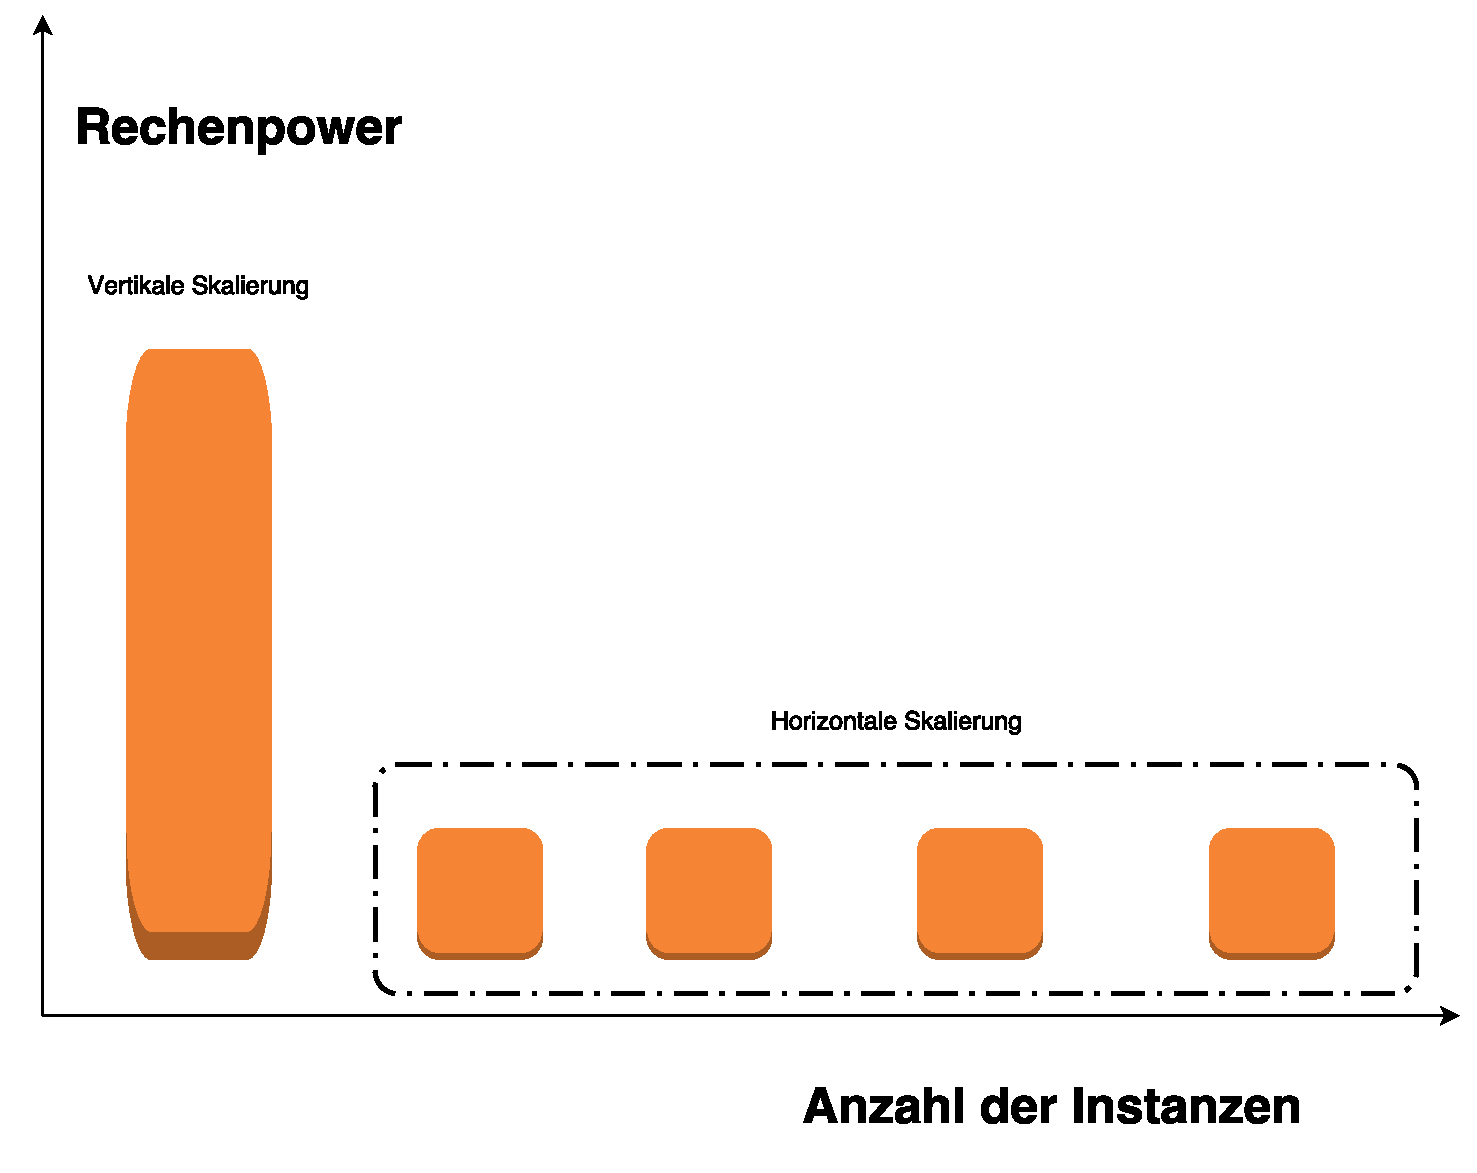
\includegraphics[width=1.0\textwidth]{figures/scalability.pdf}
    \caption{Verdeutlichung Horizontaler Skalierung}\label{fig:1}
\end{figure}
\newpage
\chapter{Übersicht über EC2-virtual-server}
\newpage
\chapter{Übersicht über EC2-container}
\newpage
\chapter{Unterschiede zwischen EC2-virtual-server und EC2-container}
\newpage
\chapter{Quellen}
\nocite{*}
\bibliography{quotes}
\bibliographystyle{plain}
\listoffigures
\end{document}
